\section{Visualization}

Three visualization tasks are considered in our work: 

\begin{enumerate}
\item Routes with tweets as exampled in Figure ~\ref{viz:social}
\item Popular routes in different cities as exampled in Figure ~\ref{viz:popularity}
\item Global workout statistic as exampled in Figure ~\ref{viz:global}
\item Recommended route preview movie as exampled in \href{http://www.cs.helsinki.fi/u/hxiao/ah/viz/route\_animation/examples/movie.html#route_path=london\_route.json}{this link}
\end{enumerate}

For the first three tasks, we used Google Maps API \footnote{https://developers.google.com/maps/}. For the last one, we use Google Street View API \footnote{https://developers.google.com/maps/documentation/streetview/}.
Some examples are shown below:


\begin{figure}[h]
\centering
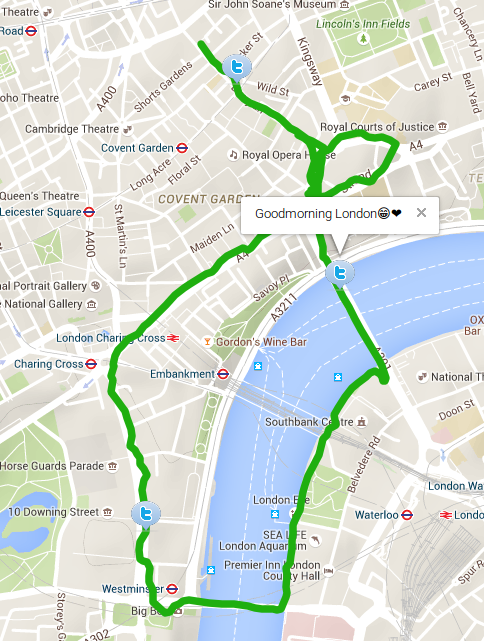
\includegraphics[width=90mm]{tweet.png}
\caption{Some running route in London annotated with location-specific tweets \label{viz:social}}
\end{figure}

\begin{figure}[h]
\centering
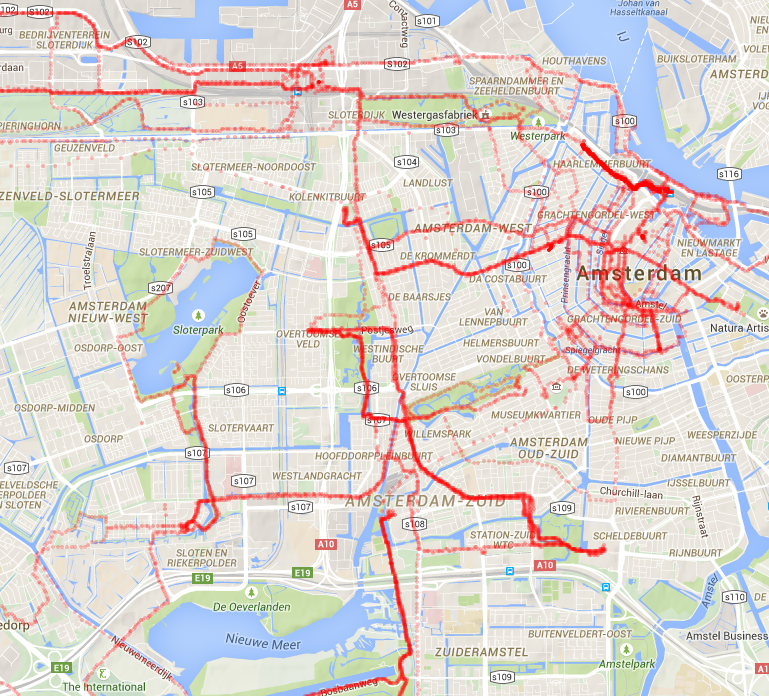
\includegraphics[width=90mm]{popularity.png}
\caption{Popularity of running routes in Amsterdam: paths with bolder color are of higher popularity  \label{viz:popularity}}
\end{figure}

\begin{figure}[h]
\centering
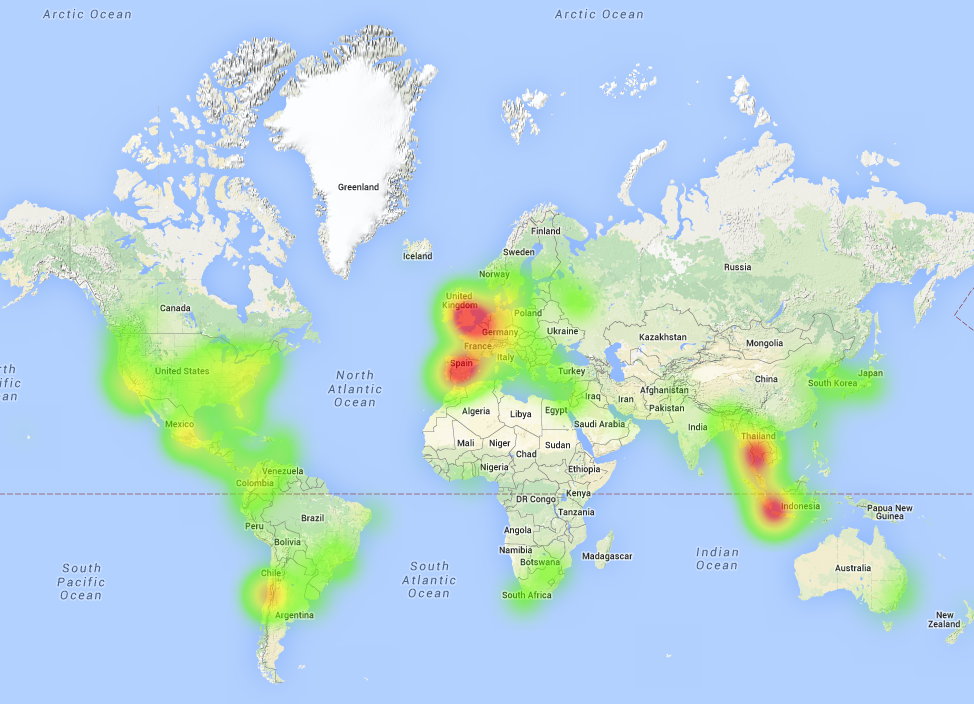
\includegraphics[width=90mm]{global.png}
\caption{Global-wise workout distance heatmap \label{viz:global}}
\end{figure}